% Draft manuscript. Every number below is a macro from generated/numbers.tex,
% produced by scripts/build_paper_numbers.py from the frozen result files.
% Do not type a result into the text. References are marked for the D-010
% verify-before-cite pass; none has been checked against its source yet.
\documentclass[conference]{IEEEtran}
\IEEEoverridecommandlockouts
\usepackage{cite}
\usepackage{amsmath,amssymb,amsfonts}
\usepackage{graphicx}
\usepackage[hidelinks]{hyperref}
\usepackage{textcomp}
\usepackage{xcolor}
\usepackage{booktabs}
\usepackage{array}
\usepackage{microtype}
% Generated by scripts/build_paper_numbers.py. Do not edit by hand.
\newcommand{\numBootDraws}{2000}
\newcommand{\numCOneDeltaZeroEight}{-0.124}
\newcommand{\numCOneDeltaZeroFive}{-0.048}
\newcommand{\numCOneDeltaZeroNine}{-0.169}
\newcommand{\numCOneDeltaZeroSeven}{-0.103}
\newcommand{\numCOneDeltaZeroSix}{-0.058}
\newcommand{\numCThreeDeltaZeroEight}{-0.088}
\newcommand{\numCThreeDeltaZeroFive}{-0.027}
\newcommand{\numCThreeDeltaZeroNine}{-0.124}
\newcommand{\numCThreeDeltaZeroSeven}{-0.069}
\newcommand{\numCThreeDeltaZeroSix}{-0.042}
\newcommand{\numCThreeUpperZeroEight}{-0.043}
\newcommand{\numCThreeUpperZeroFive}{-0.006}
\newcommand{\numCThreeUpperZeroNine}{-0.066}
\newcommand{\numCThreeUpperZeroSeven}{-0.036}
\newcommand{\numCThreeUpperZeroSix}{-0.015}
\newcommand{\numDiceCoreREight}{0.605}
\newcommand{\numDiceCoreRSeven}{0.409}
\newcommand{\numDiceCoreRTwo}{0.390}
\newcommand{\numDiceEnhREight}{0.799}
\newcommand{\numDiceEnhRSeven}{0.481}
\newcommand{\numDiceEnhRTwo}{0.431}
\newcommand{\numDiceOedREight}{0.819}
\newcommand{\numDiceOedRSeven}{0.566}
\newcommand{\numDiceOedRTwo}{0.597}
\newcommand{\numDiceREight}{0.741}
\newcommand{\numDiceRSeven}{0.485}
\newcommand{\numDiceRTwo}{0.473}
\newcommand{\numExtAbstAlphafive}{0.525}
\newcommand{\numExtAbstAlphaten}{0.243}
\newcommand{\numExtAbstAlphatwenty}{0.163}
\newcommand{\numExtAlwaysCeFlair}{0.208}
\newcommand{\numExtAlwaysDropFlair}{0.203}
\newcommand{\numExtAlwaysDropTone}{0.163}
\newcommand{\numExtAlwaysDropTonece}{0.450}
\newcommand{\numExtAlwaysDropTtwo}{0.129}
\newcommand{\numExtAlwaysFull}{0.153}
\newcommand{\numExtAurcCeFlair}{0.064}
\newcommand{\numExtAurcDropFlair}{0.101}
\newcommand{\numExtAurcDropTone}{0.058}
\newcommand{\numExtAurcDropTonece}{0.310}
\newcommand{\numExtAurcDropTtwo}{0.040}
\newcommand{\numExtAurcFull}{0.051}
\newcommand{\numExtAurcHi}{0.081}
\newcommand{\numExtAurcLo}{0.029}
\newcommand{\numExtAurcMFiveCeFlair}{0.064}
\newcommand{\numExtAurcMFiveDropFlair}{0.101}
\newcommand{\numExtAurcMFiveDropTone}{0.058}
\newcommand{\numExtAurcMFiveDropTonece}{0.310}
\newcommand{\numExtAurcMFiveDropTtwo}{0.040}
\newcommand{\numExtAurcMFiveFull}{0.051}
\newcommand{\numExtAurcMFourCeFlair}{0.270}
\newcommand{\numExtAurcMFourDropFlair}{0.175}
\newcommand{\numExtAurcMFourDropTone}{0.112}
\newcommand{\numExtAurcMFourDropTonece}{0.393}
\newcommand{\numExtAurcMFourDropTtwo}{0.173}
\newcommand{\numExtAurcMFourFull}{0.120}
\newcommand{\numExtAurcMOneCeFlair}{0.064}
\newcommand{\numExtAurcMOneDropFlair}{0.101}
\newcommand{\numExtAurcMOneDropTone}{0.058}
\newcommand{\numExtAurcMOneDropTonece}{0.310}
\newcommand{\numExtAurcMOneDropTtwo}{0.040}
\newcommand{\numExtAurcMOneFull}{0.051}
\newcommand{\numExtAurcMSixCeFlair}{0.083}
\newcommand{\numExtAurcMSixDropFlair}{0.255}
\newcommand{\numExtAurcMSixDropTone}{0.065}
\newcommand{\numExtAurcMSixDropTonece}{0.589}
\newcommand{\numExtAurcMSixDropTtwo}{0.078}
\newcommand{\numExtAurcMSixFull}{0.092}
\newcommand{\numExtAurcMThreeCeFlair}{0.065}
\newcommand{\numExtAurcMThreeDropFlair}{0.105}
\newcommand{\numExtAurcMThreeDropTone}{0.061}
\newcommand{\numExtAurcMThreeDropTonece}{0.290}
\newcommand{\numExtAurcMThreeDropTtwo}{0.039}
\newcommand{\numExtAurcMThreeFull}{0.051}
\newcommand{\numExtAurcMTwoCeFlair}{0.064}
\newcommand{\numExtAurcMTwoDropFlair}{0.101}
\newcommand{\numExtAurcMTwoDropTone}{0.058}
\newcommand{\numExtAurcMTwoDropTonece}{0.310}
\newcommand{\numExtAurcMTwoDropTtwo}{0.040}
\newcommand{\numExtAurcMTwoFull}{0.051}
\newcommand{\numExtAurocHi}{0.970}
\newcommand{\numExtAurocLo}{0.888}
\newcommand{\numExtBrierMOne}{0.118}
\newcommand{\numExtBrierMTwo}{0.121}
\newcommand{\numExtCOneDiff}{-0.025}
\newcommand{\numExtCOneHi}{0.021}
\newcommand{\numExtCOneLo}{-0.078}
\newcommand{\numExtCalCovAlphafive}{0.960}
\newcommand{\numExtCalCovAlphaten}{0.911}
\newcommand{\numExtCalCovAlphatwenty}{0.806}
\newcommand{\numExtCovAlphafive}{0.985}
\newcommand{\numExtCovAlphaten}{0.931}
\newcommand{\numExtCovAlphatwenty}{0.738}
\newcommand{\numExtDTwoAbs}{0.0034}
\newcommand{\numExtDTwoDiff}{-0.0034}
\newcommand{\numExtEFourDiff}{0.025}
\newcommand{\numExtEOneDiff}{-0.024}
\newcommand{\numExtEThreeDiff}{-0.002}
\newcommand{\numExtETwoDiff}{0.040}
\newcommand{\numExtEceMOne}{0.097}
\newcommand{\numExtEceMOneHi}{0.146}
\newcommand{\numExtEceMOneLo}{0.076}
\newcommand{\numExtEceMTwo}{0.106}
\newcommand{\numExtEceMTwoHi}{0.160}
\newcommand{\numExtEceMTwoLo}{0.091}
\newcommand{\numExtEmptyAlphafive}{0}
\newcommand{\numExtEmptyAlphaten}{0}
\newcommand{\numExtEmptyAlphatwenty}{33}
\newcommand{\numExtFullAlphafive}{106}
\newcommand{\numExtFullAlphaten}{49}
\newcommand{\numExtFullAlphatwenty}{0}
\newcommand{\numExtHalfAlphafive}{0.042}
\newcommand{\numExtHalfAlphafiveCeFlair}{0.020}
\newcommand{\numExtHalfAlphafiveDropFlair}{0.064}
\newcommand{\numExtHalfAlphafiveDropTone}{0.042}
\newcommand{\numExtHalfAlphafiveDropTonece}{0.136}
\newcommand{\numExtHalfAlphafiveDropTtwo}{0.015}
\newcommand{\numExtHalfAlphafiveFull}{0.042}
\newcommand{\numExtHalfAlphaten}{0.079}
\newcommand{\numExtHalfAlphatwenty}{0.141}
\newcommand{\numExtOracle}{0.013}
\newcommand{\numExtQuantAlphafive}{0.777}
\newcommand{\numExtQuantAlphaten}{0.662}
\newcommand{\numExtQuantAlphatwenty}{0.392}
\newcommand{\numExtREightAurc}{0.076}
\newcommand{\numExtREightAuroc}{0.927}
\newcommand{\numExtREightBrier}{0.135}
\newcommand{\numExtREightEce}{0.135}
\newcommand{\numExtRSevenAurc}{0.090}
\newcommand{\numExtRSevenAuroc}{0.904}
\newcommand{\numExtRSevenBrier}{0.137}
\newcommand{\numExtRSevenEce}{0.117}
\newcommand{\numExtRTwoAurc}{0.051}
\newcommand{\numExtRTwoAuroc}{0.929}
\newcommand{\numExtRTwoBrier}{0.121}
\newcommand{\numExtRTwoEce}{0.106}
\newcommand{\numExtRefitCovAlphafive}{0.985}
\newcommand{\numExtRefitCovAlphaten}{0.931}
\newcommand{\numExtRefitCovAlphatwenty}{0.738}
\newcommand{\numExtRiskZeroEight}{0.111}
\newcommand{\numExtRiskZeroFive}{0.030}
\newcommand{\numExtRiskZeroNine}{0.126}
\newcommand{\numExtRiskZeroSeven}{0.085}
\newcommand{\numExtRiskZeroSix}{0.066}
\newcommand{\numExtSingleTrueAlphafive}{0.969}
\newcommand{\numExtSingleTrueAlphaten}{0.908}
\newcommand{\numExtSingleTrueAlphatwenty}{0.882}
\newcommand{\numFamUAOneAdj}{0.243}
\newcommand{\numFamUAThreeAdj}{0.964}
\newcommand{\numFamUATwoAdj}{0.958}
\newcommand{\numFamUBFiveAdj}{0.263}
\newcommand{\numFamUBFourAdj}{0.267}
\newcommand{\numFamUBOneAdj}{0.985}
\newcommand{\numFamUBThreeAdj}{0.941}
\newcommand{\numFamUBTwoAdj}{0.005}
\newcommand{\numFamUDOneAdj}{0.842}
\newcommand{\numFamUDTwoAdj}{0.580}
\newcommand{\numFamUEFourAdj}{0.258}
\newcommand{\numFamUEOneAdj}{0.811}
\newcommand{\numFamUEThreeAdj}{0.811}
\newcommand{\numFamUETwoAdj}{0.748}
\newcommand{\numFamXAOneAdj}{0.960}
\newcommand{\numFamXAThreeAdj}{0.005}
\newcommand{\numFamXATwoAdj}{0.005}
\newcommand{\numFamXBFiveAdj}{0.457}
\newcommand{\numFamXBFourAdj}{0.012}
\newcommand{\numFamXBOneAdj}{0.258}
\newcommand{\numFamXBThreeAdj}{0.411}
\newcommand{\numFamXBTwoAdj}{0.005}
\newcommand{\numFamXCOneAdj}{0.457}
\newcommand{\numFamXDOneAdj}{0.411}
\newcommand{\numFamXDTwoAdj}{0.005}
\newcommand{\numFamXEFourAdj}{0.152}
\newcommand{\numFamXEOneAdj}{0.156}
\newcommand{\numFamXEThreeAdj}{0.960}
\newcommand{\numFamXETwoAdj}{0.005}
\newcommand{\numFamilyRejected}{7}
\newcommand{\numFamilySize}{29}
\newcommand{\numHdCoreREight}{6.2}
\newcommand{\numHdCoreRSeven}{11.0}
\newcommand{\numHdCoreRTwo}{9.2}
\newcommand{\numHdEnhREight}{2.0}
\newcommand{\numHdEnhRSeven}{6.0}
\newcommand{\numHdEnhRTwo}{7.5}
\newcommand{\numHdNCoreREight}{113}
\newcommand{\numHdNCoreRSeven}{121}
\newcommand{\numHdNCoreRTwo}{117}
\newcommand{\numHdNEnhREight}{91}
\newcommand{\numHdNEnhRSeven}{95}
\newcommand{\numHdNEnhRTwo}{95}
\newcommand{\numHdNOedREight}{124}
\newcommand{\numHdNOedRSeven}{124}
\newcommand{\numHdNOedRTwo}{124}
\newcommand{\numHdOedREight}{3.5}
\newcommand{\numHdOedRSeven}{9.8}
\newcommand{\numHdOedRTwo}{8.5}
\newcommand{\numIntAbstAlphafive}{0.411}
\newcommand{\numIntAbstAlphaten}{0.185}
\newcommand{\numIntAbstAlphatwenty}{0.121}
\newcommand{\numIntAlwaysCeFlair}{0.218}
\newcommand{\numIntAlwaysDropFlair}{0.226}
\newcommand{\numIntAlwaysDropTone}{0.177}
\newcommand{\numIntAlwaysDropTonece}{0.532}
\newcommand{\numIntAlwaysDropTtwo}{0.185}
\newcommand{\numIntAlwaysFull}{0.218}
\newcommand{\numIntAurcCeFlair}{0.113}
\newcommand{\numIntAurcDropFlair}{0.108}
\newcommand{\numIntAurcDropTone}{0.076}
\newcommand{\numIntAurcDropTonece}{0.493}
\newcommand{\numIntAurcDropTtwo}{0.073}
\newcommand{\numIntAurcFull}{0.076}
\newcommand{\numIntAurcHi}{0.123}
\newcommand{\numIntAurcLo}{0.041}
\newcommand{\numIntAurcMFiveCeFlair}{0.113}
\newcommand{\numIntAurcMFiveDropFlair}{0.108}
\newcommand{\numIntAurcMFiveDropTone}{0.076}
\newcommand{\numIntAurcMFiveDropTonece}{0.493}
\newcommand{\numIntAurcMFiveDropTtwo}{0.073}
\newcommand{\numIntAurcMFiveFull}{0.076}
\newcommand{\numIntAurcMFourCeFlair}{0.124}
\newcommand{\numIntAurcMFourDropFlair}{0.112}
\newcommand{\numIntAurcMFourDropTone}{0.071}
\newcommand{\numIntAurcMFourDropTonece}{0.370}
\newcommand{\numIntAurcMFourDropTtwo}{0.079}
\newcommand{\numIntAurcMFourFull}{0.080}
\newcommand{\numIntAurcMOneCeFlair}{0.113}
\newcommand{\numIntAurcMOneDropFlair}{0.108}
\newcommand{\numIntAurcMOneDropTone}{0.076}
\newcommand{\numIntAurcMOneDropTonece}{0.493}
\newcommand{\numIntAurcMOneDropTtwo}{0.073}
\newcommand{\numIntAurcMOneFull}{0.076}
\newcommand{\numIntAurcMSixCeFlair}{0.133}
\newcommand{\numIntAurcMSixDropFlair}{0.308}
\newcommand{\numIntAurcMSixDropTone}{0.085}
\newcommand{\numIntAurcMSixDropTonece}{0.723}
\newcommand{\numIntAurcMSixDropTtwo}{0.141}
\newcommand{\numIntAurcMSixFull}{0.134}
\newcommand{\numIntAurcMThreeCeFlair}{0.117}
\newcommand{\numIntAurcMThreeDropFlair}{0.106}
\newcommand{\numIntAurcMThreeDropTone}{0.080}
\newcommand{\numIntAurcMThreeDropTonece}{0.473}
\newcommand{\numIntAurcMThreeDropTtwo}{0.075}
\newcommand{\numIntAurcMThreeFull}{0.080}
\newcommand{\numIntAurcMTwoCeFlair}{0.113}
\newcommand{\numIntAurcMTwoDropFlair}{0.108}
\newcommand{\numIntAurcMTwoDropTone}{0.076}
\newcommand{\numIntAurcMTwoDropTonece}{0.493}
\newcommand{\numIntAurcMTwoDropTtwo}{0.073}
\newcommand{\numIntAurcMTwoFull}{0.076}
\newcommand{\numIntAurocHi}{0.956}
\newcommand{\numIntAurocLo}{0.801}
\newcommand{\numIntBrierMOne}{0.140}
\newcommand{\numIntBrierMTwo}{0.139}
\newcommand{\numIntCalCovAlphafive}{0.960}
\newcommand{\numIntCalCovAlphaten}{0.911}
\newcommand{\numIntCalCovAlphatwenty}{0.806}
\newcommand{\numIntCovAlphafive}{0.960}
\newcommand{\numIntCovAlphaten}{0.871}
\newcommand{\numIntCovAlphatwenty}{0.726}
\newcommand{\numIntEceMOne}{0.119}
\newcommand{\numIntEceMOneHi}{0.190}
\newcommand{\numIntEceMOneLo}{0.087}
\newcommand{\numIntEceMTwo}{0.122}
\newcommand{\numIntEceMTwoHi}{0.194}
\newcommand{\numIntEceMTwoLo}{0.090}
\newcommand{\numIntEmptyAlphafive}{0}
\newcommand{\numIntEmptyAlphaten}{0}
\newcommand{\numIntEmptyAlphatwenty}{15}
\newcommand{\numIntFullAlphafive}{51}
\newcommand{\numIntFullAlphaten}{23}
\newcommand{\numIntFullAlphatwenty}{0}
\newcommand{\numIntHalfAlphafive}{0.077}
\newcommand{\numIntHalfAlphafiveCeFlair}{0.081}
\newcommand{\numIntHalfAlphafiveDropFlair}{0.077}
\newcommand{\numIntHalfAlphafiveDropTone}{0.077}
\newcommand{\numIntHalfAlphafiveDropTonece}{0.222}
\newcommand{\numIntHalfAlphafiveDropTtwo}{0.065}
\newcommand{\numIntHalfAlphafiveFull}{0.077}
\newcommand{\numIntHalfAlphaten}{0.097}
\newcommand{\numIntHalfAlphatwenty}{0.129}
\newcommand{\numIntOracle}{0.027}
\newcommand{\numIntQuantAlphafive}{0.777}
\newcommand{\numIntQuantAlphaten}{0.662}
\newcommand{\numIntQuantAlphatwenty}{0.392}
\newcommand{\numIntREightAurc}{0.097}
\newcommand{\numIntREightAuroc}{0.889}
\newcommand{\numIntREightBrier}{0.153}
\newcommand{\numIntREightEce}{0.173}
\newcommand{\numIntRSevenAurc}{0.093}
\newcommand{\numIntRSevenAuroc}{0.888}
\newcommand{\numIntRSevenBrier}{0.129}
\newcommand{\numIntRSevenEce}{0.109}
\newcommand{\numIntRTwoAurc}{0.076}
\newcommand{\numIntRTwoAuroc}{0.878}
\newcommand{\numIntRTwoBrier}{0.139}
\newcommand{\numIntRTwoEce}{0.122}
\newcommand{\numIntRefitCovAlphafive}{0.960}
\newcommand{\numIntRefitCovAlphaten}{0.871}
\newcommand{\numIntRefitCovAlphatwenty}{0.726}
\newcommand{\numIntRiskZeroEight}{0.160}
\newcommand{\numIntRiskZeroFive}{0.048}
\newcommand{\numIntRiskZeroNine}{0.170}
\newcommand{\numIntRiskZeroSeven}{0.115}
\newcommand{\numIntRiskZeroSix}{0.093}
\newcommand{\numIntSingleTrueAlphafive}{0.932}
\newcommand{\numIntSingleTrueAlphaten}{0.842}
\newcommand{\numIntSingleTrueAlphatwenty}{0.826}
\newcommand{\numNExt}{202}
\newcommand{\numNExtPos}{80}
\newcommand{\numNInt}{124}
\newcommand{\numNIntPos}{35}
\newcommand{\numPermDraws}{10000}
\newcommand{\numPrevExt}{0.396}
\newcommand{\numPrevInt}{0.282}
\newcommand{\numProbeAuroc}{0.787}
\newcommand{\numProbeAurocHi}{0.919}
\newcommand{\numProbeAurocLo}{0.627}
\newcommand{\numProbeCodel}{14}
\newcommand{\numProbeIdhAuroc}{0.714}
\newcommand{\numProbeMutAuroc}{0.673}
\newcommand{\numProbeMutAurocHi}{0.870}
\newcommand{\numProbeMutAurocLo}{0.441}
\newcommand{\numProbeMutIdhAuroc}{0.337}
\newcommand{\numProbeMutN}{28}
\newcommand{\numProbeN}{66}
\newcommand{\numProbeTrainCodel}{37}
\newcommand{\numProbeTrainN}{193}
\newcommand{\numStatusCFiveExt}{supported}
\newcommand{\numStatusCFiveInt}{inconclusive}
\newcommand{\numStatusCFourExt}{refuted}
\newcommand{\numStatusCFourInt}{refuted}
\newcommand{\numStatusCOneExt}{not applicable}
\newcommand{\numStatusCOneInt}{supported}
\newcommand{\numStatusCSixExt}{inconclusive}
\newcommand{\numStatusCSixInt}{refuted}
\newcommand{\numStatusCThreeExt}{supported}
\newcommand{\numStatusCThreeInt}{not evaluated}
\newcommand{\numStatusCThreeWorst}{inconclusive}
\newcommand{\numStatusCTwoExt}{not applicable}
\newcommand{\numStatusCTwoInt}{refuted}
\newcommand{\numTemperature}{1.125}


\begin{document}

\title{Calibrated Selective Prediction for MRI-Based Glioma IDH Classification under Missing Modalities and Cross-Institutional Domain Shift}

% Author list and affiliations are not decided (PROJECT_STATE, paper parked).
\author{
\begin{tabular}{c}
\textbf{Aniket Saha}\\
Department of Computer Science \\
and Engineering\\
\textit{Lovely Professional University}\\
Phagwara, Punjab\\
aniketsahaworkspace@gmail.com
\end{tabular}
}

\maketitle

\begin{abstract}
% Anchored on the SPEC 8.3 sentence. The word "first" is deliberately absent:
% it ships only after the dated novelty check (D-010, PUBLICATION_PLAN 2).
We provide a systematic risk--coverage analysis and an empirical characterisation of conformal coverage for inference-time calibrated selective prediction in MRI-based glioma IDH classification. The question is tested, not assumed: does abstaining on low-confidence cases improve reliability, and does conformal coverage stay close to nominal, under missing MRI sequences and cross-institutional shift? A segmentation-assisted 3D network was trained on UTSW-Glioma and evaluated on its held-out test split ($n=\numNInt$) and, once, on UCSF-PDGM ($n=\numNExt$), with temperature scaling, Monte Carlo dropout, a five-member ensemble and split conformal prediction as abstention mechanisms, and with sequences removed at inference. On complete input, abstaining lowered selective risk below the always-predict risk at every coverage level on both cohorts; on UCSF-PDGM the risk at coverage 0.5 was \numExtRiskZeroFive{} against \numExtAlwaysFull{}. Four of the six pre-registered claims were not supported in at least one cohort. The advantage was lost when T1 contrast-enhanced (T1ce) was removed (C2 refuted internally), conformal coverage could not be characterised within the pre-registered tolerance because the intervals at these sample sizes are wider than the band (C4 refuted on both cohorts), and abstention was not enriched for errors under T1ce removal (C6 refuted internally). Temperature scaling did not lower expected calibration error on either cohort. We report these as negative results. The analysis was pre-registered, the external evaluation was run once under a signed freeze manifest, and every number in the text is generated from frozen result files.
\end{abstract}

\begin{IEEEkeywords}
Glioma, IDH mutation, selective prediction, conformal prediction, calibration, missing modalities, domain shift.
\end{IEEEkeywords}

\section{Introduction}

IDH mutation status drives diagnosis, prognosis and treatment planning for diffuse glioma under the WHO 2021 classification \cite{louis2021}. Obtaining it from a biopsy is invasive, so a model that predicts it from a preoperative MRI is attractive. A model that outputs a confident-looking probability for every scan is also risky. When one of the usual sequences is missing, or the scan comes from a different hospital than the training data, its confidence often stops tracking its accuracy, and it can be wrong while sounding sure.

This study asks a narrower question than ``how accurate is the model.'' Instead of forcing an answer for every case, can the classifier recognise when it should not answer and flag the case for a clinician or a laboratory test, in the two situations where MRI models are known to struggle: missing sequences and scans from another institution? Formally, a selective classifier $(f,g)$ pairs a probability estimator $f$ with an accept/abstain rule $g$. Coverage $\phi$ is the fraction of cases accepted and selective risk is the error rate on those cases. The risk--coverage curve traces selective risk as the threshold moves, and AURC is the area under it \cite{geifman2017}. We evaluate $(f,g)$ for complete and simulated missing MRI, on an internal and an external cohort, and measure how far the empirical coverage of a conformal rule drifts from its nominal level. The conformal guarantee assumes exchangeability between calibration and test data \cite{vovk2005,angelopoulos2023}, which domain shift and missing sequences violate. We do not assume it holds. The size and pattern of the deviation is what we measure.

The nearest glioma studies have solved the pieces separately (Section~II): discrimination is strong, missing-sequence handling exists, and calibration or a single conformal operating point has been reported. Among the five closest studies we identified, none follows the abstention decision itself through both missing sequences and an external cohort. This paper is an empirical trustworthiness study. It does not propose an architecture, and the backbone is not a contribution.

\subsection{Objectives}
We ask, for MRI-based IDH classification: (RQ1) under missing sequences and cross-institutional shift, does a calibrated selective mechanism give a well-behaved risk--coverage trade-off, so that rejecting low-confidence cases lowers selective risk and AURC relative to always predicting; (RQ2) does empirical coverage stay close to nominal, and how does breaking exchangeability affect it; (RQ3) does calibration degrade from internal to external data; and (RQ4, exploratory) does the same behaviour hold for 1p/19q codeletion given its small label count.

\subsection{Contributions}
\begin{itemize}
\item A pre-registered risk--coverage and coverage-deviation analysis of five abstention mechanisms across six input conditions on an internal and an external cohort.
\item Six falsifiable claims, each with a fixed rule for supported, refuted and inconclusive, written before any external result was seen. We report which ones failed.
\item A single external evaluation under a signed freeze manifest, with the analysis code tested on synthetic data first.
\item A multiplicity-controlled family of $\numFamilySize$ comparisons (Benjamini--Hochberg, $q=0.05$), of which $\numFamilyRejected$ are rejected.
\end{itemize}

\section{Related Work}

\subsection{Glioma IDH prediction}
\textbf{Elyassirad et al.}\ are the closest study \cite{elyassirad2026}. They train on UCSF and test on UPenn with complete sequences, and abstain at a single fixed conformal operating point. We add the full risk--coverage sweep, AURC, the missing-sequence axis, and the calibration metrics they do not report. \textbf{Liu et al.} (GMMAS) use uncertainty to filter pseudo-labels during training, never to gate an inference-time decision, and test no abstention, risk--coverage curve or coverage level \cite{liu2026gmmas}. \textbf{Yogananda et al.} work on the same cohort family (UTSW, UCSF, EGD) and derive a confidence score from a Bayesian logistic regression \cite{yogananda2025}; we differ in mechanism, testing abstention and risk--coverage, and they list missing sequences as an unaddressed limitation. \textbf{Liang et al.} (RISEN) estimate missing sequences by imputation and then always predict \cite{liang2026risen}; we zero the missing sequence and allow the model to abstain. \textbf{Farahani et al.} (FoundBioNet) set a discrimination ceiling with a tumour-aware foundation-style network and report neither uncertainty nor calibration \cite{farahani2025}. We approach that accuracy only as far as needed to make the trust mechanism meaningful.

Across these studies, discrimination, missing-sequence robustness and point-estimate calibration have each been addressed. We found none that turns uncertainty into an inference-time decision to withhold a prediction and then tests whether that decision stays trustworthy under both missing sequences and external shift.

\subsection{Selective and conformal prediction under shift}
Selective classification trades coverage for risk \cite{geifman2017}, and post-hoc confidence can reduce reliance on expert review even in segmentation under shift \cite{borges2024}. For classification, Hirsch and Goldberger learn an instance-dependent conformal threshold and then conformalise it, shrinking average set size at the requested coverage \cite{hirsch2024}. Lu et al.\ replace exchangeability with partial exchangeability for federated clients \cite{lu2023}, and Cheung et al.\ extend conformal bounds to reconstruction metrics rather than labels \cite{cheung2024}. These works motivate a post-hoc trust layer that can abstain, return a set, or bound an error, and each names the assumption that must be checked: calibration coverage, shift, site heterogeneity, and fit between the uncertainty target and the clinical decision. The trade can also fail. Selective classification has been analysed formally under covariate and label shift \cite{liang2024selective}, and Zadorozhny et al.\ show non-monotone referral curves and large error rises at high referral rates on retinal and chest images \cite{zadorozhny2023}. Our monotonicity claim (C5) tests that failure on glioma MRI instead of assuming it. Temperature scaling is the standard post-hoc calibration fix \cite{guo2017}; Monte Carlo dropout and deep ensembles supply alternative uncertainty scores \cite{gal2016,lakshminarayanan2017}; split conformal prediction and conformal risk control give a distribution-free target under exchangeability \cite{vovk2005,angelopoulos2023,angelopoulos2024crc}. We use the conformal target as a fixed number to measure deviations against.

\subsection{Cohort overlap and leakage}
Public brain-tumour benchmarks are not automatically independent. BraTS 2021 contains studies from TCGA-GBM, TCGA-LGG, IvyGAP and CPTAC-GBM \cite{dorfner2025}, so a cross-dataset test can place one patient on both sides unless source identifiers are reconciled. Ren et al.\ excluded patients overlapping between BraTS 2021 and the TCGA and UPenn collections before pooling five public glioma datasets \cite{ren2025}; Liu et al.\ matched identifiers and metadata, added perceptual hashing for near-identical images, and assigned each subject to one split \cite{liu2026dare}. Leakage also arises inside one collection: slice-level splits inflated brain-MRI classification accuracy by 29 to 55\% relative to subject-level splits in one study \cite{yagis2021}. We split by patient and, for the external cohort, excluded patients who also appear in BraTS 2021.

\section{Materials and Methods}

\subsection{Cohorts and splits}
UTSW-Glioma \cite{reddy2026utsw} is the only development cohort. After quality control, 616 of 625 patients remained (three without an IDH label, six with a failed skull-strip check). IDH labels in this cohort come from two assays: 413 of 622 labelled patients (66\%) by immunohistochemistry, which can miss non-R132H variants and so label them wildtype, and 209 (34\%) by sequencing. Label definitions across cohorts were harmonised by one reviewer without an independent cross-check.

We split at the patient level, stratified on IDH only, into 60/20/20 train, calibration and internal-test sets with a seed fixed before the split was inspected. Per-class rounding gives 103 mutant and 265 wildtype patients in training (368) and 35 mutant and 89 wildtype in each of the calibration and internal-test splits (124 each). The 1p/19q categories are reported per split but not used for stratification. A power simulation run before the split showed that at this test size the 95\% bootstrap AUROC half-width is about 0.09 at a true AUROC of 0.75 and 0.06 at 0.90 (Hanley--McNeil intervals are wider), and that no feasible calibration size on this cohort brings the coverage-deviation half-width below five percentage points, while a five-point coverage grid from 0.5 to 0.9 remains usable. The internal-test split holds $\numNIntPos$ mutant patients of $\numNInt$ (prevalence $\numPrevInt$).

UCSF-PDGM \cite{calabrese2022ucsf} is an external test cohort that is never split or used for development. Of 501 patients, 293 were excluded because they also appear in BraTS 2021 and 6 had no imaging, leaving $\numNExt$ patients ($\numNExtPos$ mutant, prevalence $\numPrevExt$). Its IDH assay was not independently re-confirmed against the original publication. The overlap exclusion shifts the label mix, so internal and external accuracy are not directly comparable. A third cohort (EGD) is deferred to a later, separately frozen evaluation.

\subsection{Preprocessing}
For each patient the four structural sequences (T1, T1ce, T2, FLAIR) were rigidly registered to T1ce, skull-stripped with HD-BET \cite{isensee2019hdbet}, bias-corrected with N4 \cite{tustison2010n4}, and resampled to about 1\,mm isotropic spacing. Raw intensity scales differ widely between patients (in the training dry run the per-patient mean T1 brain intensity ranged from 123 to 271\,321 around a median of about 565, and 7\% of patients had a modality above 5\,000), so each volume was first divided by its own positive brain-voxel median. Per-modality mean and population standard deviation were then computed from the 368 training patients' brain voxels in float64 and applied unchanged to every split and cohort. Background stays exactly zero and nothing is clipped. External volumes therefore need no statistics of their own.

\subsection{Model and training}
The classifier is a MONAI SegResNet \cite{myronenko2019segresnet,cardoso2022monai} (32 initial filters, encoder blocks $[1,2,2,4]$) with an auxiliary three-class segmentation head (enhancing tumour, non-enhancing core, oedema). Features are pooled inside the predicted tumour region and passed to a small classification head (64 hidden units, dropout 0.2). Training used AdamW \cite{loshchilov2019adamw} (learning rate $3\times10^{-4}$, weight decay $10^{-4}$), batch size 2 with four-step accumulation, bf16, gradient clipping at 1.0, up to 300 epochs with early stopping (patience 30) on the class-balanced classification loss of the calibration split, and a mutant-class weight of 2.57. Modality dropout was applied during training: all four sequences were kept with probability 0.5, otherwise some sequences were zeroed. Nothing in the architecture or training recipe was searched over.

Five seeds were trained (R2 to R6). R2 is the primary model; R2 to R6 form the ensemble. Two pre-specified variants were also trained for ablation: R7 (global average pooling instead of tumour-aware pooling) and R8 (two independent networks, a segmentation network followed by a classifier that pools inside its frozen mask). A comparator, R1, uses R2's architecture but no modality dropout.

\subsection{Missing sequences}
Missing sequences were simulated at inference by setting the removed channels to zero. Nothing was imputed. The six conditions are full input, removal of each of T1, T1ce, T2 and FLAIR, and T1ce+FLAIR only.

\subsection{Abstention mechanisms}
Each mechanism assigns a confidence to each patient; the model abstains on the least confident cases.
\begin{itemize}
\item \textbf{M1, M2:} $\max(p,1-p)$ for the raw and the temperature-scaled probability of IDH mutation. The temperature $T=\numTemperature$ was fitted once on the UTSW calibration split and never refitted on any other data.
\item \textbf{M3:} negative predictive entropy of 30 Monte Carlo passes through the dropout layers of the head.
\item \textbf{M4:} negative variance of the five ensemble members' probabilities.
\item \textbf{M5:} split conformal prediction with nonconformity $1-p(\text{true class})$ on the scaled probability. The quantile for miscoverage $\alpha\in\{0.05,0.1,0.2\}$ is the $\lceil (n+1)(1-\alpha)\rceil$-th smallest calibration score and is carried over unchanged to every condition and cohort.
\item \textbf{M6:} the comparator R1 with raw confidence.
\end{itemize}
M1, M2 and M5 rank patients identically, because temperature scaling is monotone; they differ in operating points and in prediction-set coverage.

\subsection{Metrics}
Selective risk at coverage $\phi$ is the error rate on the $\phi$ fraction of most-confident patients. The risk--coverage curve plots it against $\phi$, and AURC is its mean over all cutoffs. We evaluate $\phi\in\{0.5,0.6,0.7,0.8,0.9\}$ and compare with the always-predict risk. Calibration uses ECE (10 equal-width bins) and the Brier score; discrimination uses AUROC with the Hanley--McNeil interval \cite{hanley1982}. AUROC is never reported without ECE, Brier, AURC and coverage beside it. Coverage deviation is empirical minus nominal set coverage, with a two-stage bootstrap interval over calibration and test patients.

\subsection{Pre-registered claims and decision rules}
Six claims were fixed before any external result. C1: selective prediction beats always-predict internally. C2: that advantage survives missing sequences. C3: it survives external shift. C4: coverage deviation can be characterised within a $\pm0.07$ band. C5: risk--coverage curves are monotone. C6: abstention is enriched for errors. With $D(\phi)$ the selective minus always-predict risk, C1 to C3 are refuted if any point estimate of $D$ is $\ge0$, supported if every upper 95\% limit is below 0, and inconclusive otherwise. C4 is refuted if any condition's coverage-deviation interval has half-width above $0.07$. C5 is refuted if any adjacent-coverage lower limit is above 0 and supported if every point difference is $\le0$. C6 is refuted if any observed enrichment is $\le0$ and supported if every BH-adjusted permutation $p$ is below $0.05$. The worst status over conditions decides the claim. Refutations are reported as refutations.

\subsection{Statistics and multiplicity}
Intervals use $\numBootDraws$ bootstrap draws over patients with one shared index matrix; permutation tests use $\numPermDraws$ draws; AUROC differences use DeLong's test \cite{delong1988}. The confirmatory family has $\numFamilySize$ comparisons (14 on UTSW, 15 on UCSF-PDGM: mechanism contrasts, missing-sequence contrasts, internal versus external, calibration contrasts and ablations), adjusted once with Benjamini--Hochberg at $q=0.05$ \cite{benjamini1995}. The family is 29 rather than the 44 pre-registered with EGD because EGD is deferred.

\subsection{Protocol integrity}
The external cohort was evaluated once, through a harness that refuses to run without a signed freeze manifest naming the exact model checkpoints, calibration parameters and code commit, and that re-checks the repository state after the run. The manifest initially omitted R7 and R8; this was found before any external metric was examined and corrected with a second signed manifest and run, with no change to any method. External analysis code was written and tested on synthetic data before it saw real predictions. A second agent recomputed the external numbers independently from the written contracts (Section~\ref{sec:limits}).

\section{Results}

\subsection{Complete input}
Table~\ref{tab:main} gives discrimination, calibration and AURC. On the internal test split the primary model reached an AUROC of \numIntRTwoAuroc{} (95\% interval \numIntAurocLo{} to \numIntAurocHi{}), and on UCSF-PDGM \numExtRTwoAuroc{} (\numExtAurocLo{} to \numExtAurocHi{}). The external value is higher; prevalence and case mix differ, so we do not read it as better generalisation.

\begin{table}[t]
\centering
\caption{Primary model and ablations on complete input (temperature-scaled ECE and Brier; AURC as mean over cutoffs).}
\label{tab:main}
\begin{tabular}{llcccc}
\toprule
Cohort & Model & AUROC & ECE & Brier & AURC \\
\midrule
UTSW test & R2 & \numIntRTwoAuroc & \numIntRTwoEce & \numIntRTwoBrier & \numIntRTwoAurc \\
UTSW test & R7 & \numIntRSevenAuroc & \numIntRSevenEce & \numIntRSevenBrier & \numIntRSevenAurc \\
UTSW test & R8 & \numIntREightAuroc & \numIntREightEce & \numIntREightBrier & \numIntREightAurc \\
UCSF-PDGM & R2 & \numExtRTwoAuroc & \numExtRTwoEce & \numExtRTwoBrier & \numExtRTwoAurc \\
UCSF-PDGM & R7 & \numExtRSevenAuroc & \numExtRSevenEce & \numExtRSevenBrier & \numExtRSevenAurc \\
UCSF-PDGM & R8 & \numExtREightAuroc & \numExtREightEce & \numExtREightBrier & \numExtREightAurc \\
\bottomrule
\end{tabular}
\end{table}

\subsection{Does abstaining lower risk? (RQ1, C1, C3)}
Table~\ref{tab:risk} shows selective risk by coverage. Internally the always-predict risk was \numIntAlwaysFull{} and the risk fell to \numIntRiskZeroFive{} at coverage 0.5. Externally the always-predict risk was \numExtAlwaysFull{} and the risk fell to \numExtRiskZeroFive{}. Every upper 95\% limit of $D(\phi)$ was below zero on the external full-input condition, so C3 is supported there (\numCThreeDeltaZeroNine{} at coverage 0.9 and \numCThreeDeltaZeroFive{} at 0.5). C1 is supported internally.

\begin{table}[t]
\centering
\caption{Selective risk of the primary model at target coverage (full input), with always-predict risk.}
\label{tab:risk}
\begin{tabular}{lcccccc}
\toprule
Cohort & 0.5 & 0.6 & 0.7 & 0.8 & 0.9 & Always \\
\midrule
UTSW test & \numIntRiskZeroFive & \numIntRiskZeroSix & \numIntRiskZeroSeven & \numIntRiskZeroEight & \numIntRiskZeroNine & \numIntAlwaysFull \\
UCSF-PDGM & \numExtRiskZeroFive & \numExtRiskZeroSix & \numExtRiskZeroSeven & \numExtRiskZeroEight & \numExtRiskZeroNine & \numExtAlwaysFull \\
\bottomrule
\end{tabular}
\end{table}

The mechanisms differ little on complete input. M1, M2 and M5 rank identically, and the contrast with MC dropout was not different from zero after adjustment (UCSF-PDGM adjusted $p=\numFamXAOneAdj$). The ensemble variance ranking was worse than the confidence ranking on UCSF-PDGM (adjusted $p=\numFamXATwoAdj$). Conformal risk control therefore adds no ranking advantage over temperature-scaled confidence; its contribution is a coverage target, examined below.

\subsection{Missing sequences (RQ1, C2, C5)}
Removing T1ce had the largest effect. Table~\ref{tab:missing} and Fig.~\ref{fig:rc} show AURC and the curves against always-predict risk. With T1ce removed, the internal AURC was \numIntAurcDropTonece{} against an always-predict risk of \numIntAlwaysDropTonece{}, and D($\phi$) was not below zero at every coverage level, so C2 is refuted. The external AURC with T1ce removed was \numExtAurcDropTonece{} against \numExtAlwaysDropTonece{}. Its increase over full input is one of the rejected family members on both cohorts (internal adjusted $p=\numFamUBTwoAdj$, external $p=\numFamXBTwoAdj$). Removing FLAIR also raised the external AURC, by less (adjusted $p=\numFamXBFourAdj$); removing T1 or T2 changed little. Risk--coverage curves were monotone in every external condition (C5 supported) and inconclusive internally.

\begin{table}[t]
\centering
\caption{AURC and always-predict risk by input condition (primary model). Missing-sequence conditions ($-$T1 and below) are simulated by zeroing channels.}
\label{tab:missing}
\begin{tabular}{lcccc}
\toprule
 & \multicolumn{2}{c}{UTSW test} & \multicolumn{2}{c}{UCSF-PDGM} \\
Condition & AURC & Always & AURC & Always \\
\midrule
Full & \numIntAurcFull & \numIntAlwaysFull & \numExtAurcFull & \numExtAlwaysFull \\
$-$T1 & \numIntAurcDropTone & \numIntAlwaysDropTone & \numExtAurcDropTone & \numExtAlwaysDropTone \\
$-$T1ce & \numIntAurcDropTonece & \numIntAlwaysDropTonece & \numExtAurcDropTonece & \numExtAlwaysDropTonece \\
$-$T2 & \numIntAurcDropTtwo & \numIntAlwaysDropTtwo & \numExtAurcDropTtwo & \numExtAlwaysDropTtwo \\
$-$FLAIR & \numIntAurcDropFlair & \numIntAlwaysDropFlair & \numExtAurcDropFlair & \numExtAlwaysDropFlair \\
T1ce+FLAIR & \numIntAurcCeFlair & \numIntAlwaysCeFlair & \numExtAurcCeFlair & \numExtAlwaysCeFlair \\
\bottomrule
\end{tabular}
\end{table}

\begin{figure*}[t]
\centering
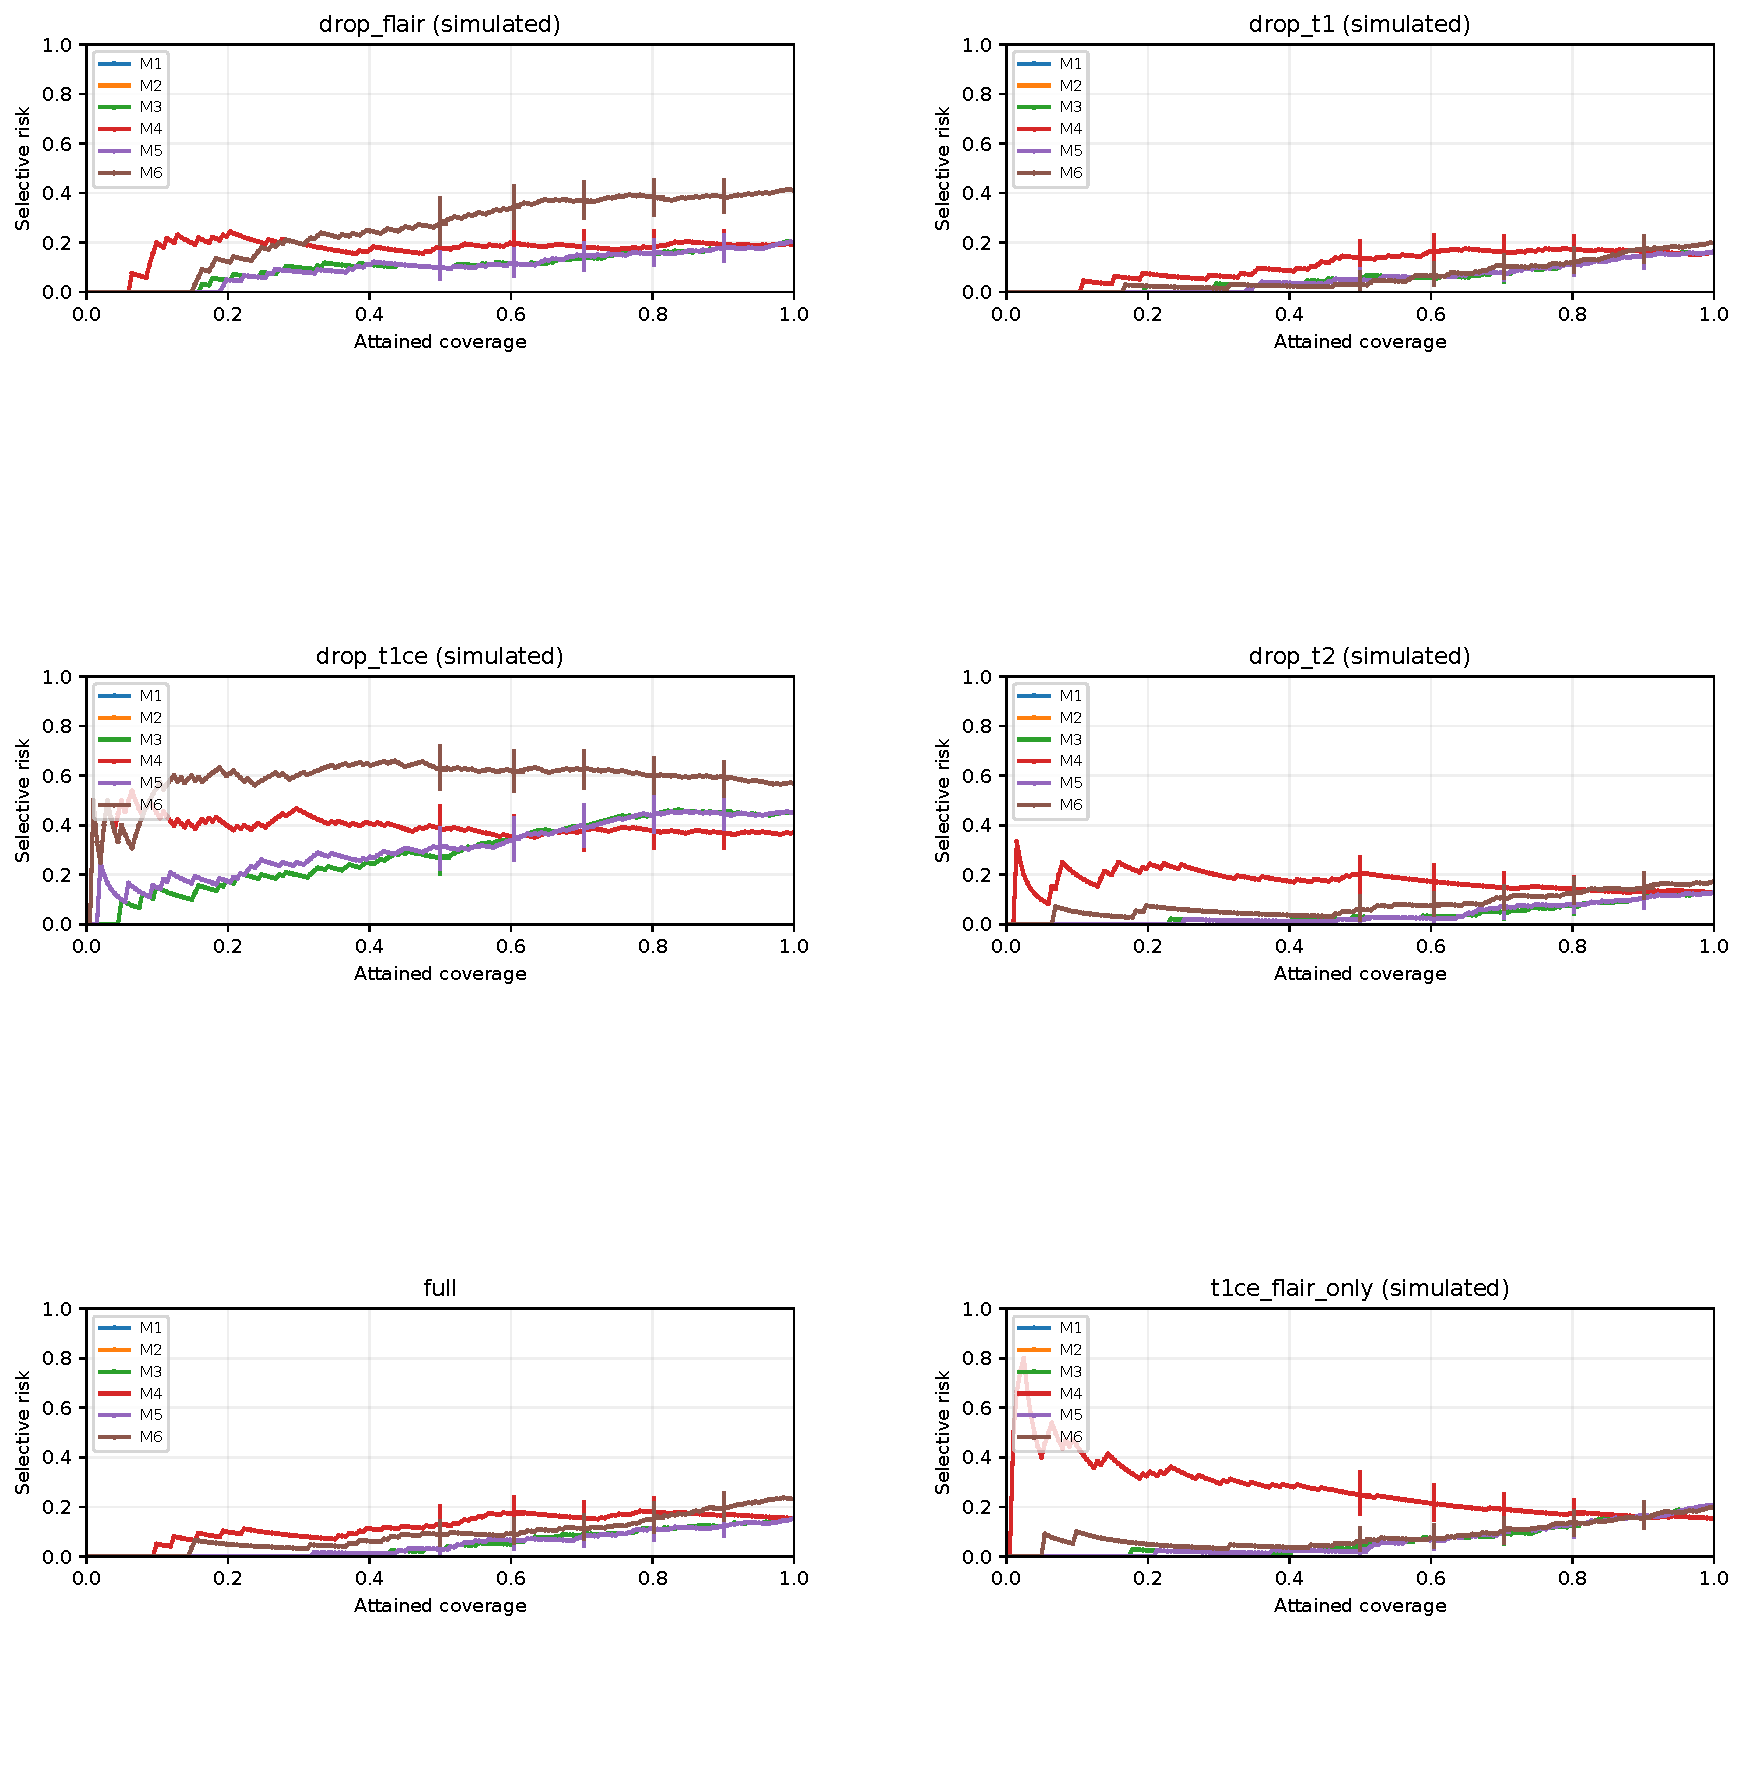
\includegraphics[width=0.85\textwidth]{figures/fig_2_ucsf_pdgm.pdf}
\caption{Risk--coverage curves on UCSF-PDGM for each input condition (simulated missing sequences) and mechanism M1 to M6. Vertical bars are 95\% intervals at the five evaluated coverage levels.}
\label{fig:rc}
\end{figure*}

\subsection{Is abstention enriched for errors? (C6)}
On the external cohort the rejected cases had a higher error rate than the cohort average at every coverage level, and the BH-adjusted permutation $p$ was below 0.05 in four of six conditions. The two exceptions (T1 removed, T1ce removed) are inconclusive, so the external claim is \numStatusCSixExt. Internally, with T1ce removed, the observed enrichment was at or below zero at every coverage level, so C6 is refuted internally.

\subsection{Does conformal coverage hold? (RQ2, C4)}
\label{sec:coverage}
Table~\ref{tab:cov} gives set coverage on the full-input condition and Fig.~\ref{fig:cov} shows it for every condition. At $\alpha=0.05$ the external coverage was \numExtCovAlphafive{} against a nominal 0.95, inside the $\pm0.07$ band. At $\alpha=0.2$ it was \numExtCovAlphatwenty{} against 0.80, and \numExtEmptyAlphatwenty{} of the $\numNExt$ prediction sets were empty. On the external cohort the interval half-width exceeded $0.07$ in every condition at $\alpha=0.1$ and $0.2$; at $\alpha=0.05$ five of six conditions passed and T1ce removal did not (half-width \numExtHalfAlphafiveDropTonece). Internally, all but one of the condition--$\alpha$ cells exceeded the band. C4 is therefore refuted: at these sample sizes the intervals cannot separate preserved from degraded coverage. This is a statement about the precision of the measurement, not a finding that coverage holds or fails.

\begin{table}[t]
\centering
\caption{Conformal set coverage, full input, quantiles from the UTSW calibration split. Half-width is that of the coverage-deviation interval.}
\label{tab:cov}
\begin{tabular}{lccccc}
\toprule
 & & \multicolumn{2}{c}{UTSW test} & \multicolumn{2}{c}{UCSF-PDGM} \\
$\alpha$ & Nominal & Cov. & Half & Cov. & Half \\
\midrule
0.05 & 0.95 & \numIntCovAlphafive & \numIntHalfAlphafive & \numExtCovAlphafive & \numExtHalfAlphafive \\
0.10 & 0.90 & \numIntCovAlphaten & \numIntHalfAlphaten & \numExtCovAlphaten & \numExtHalfAlphaten \\
0.20 & 0.80 & \numIntCovAlphatwenty & \numIntHalfAlphatwenty & \numExtCovAlphatwenty & \numExtHalfAlphatwenty \\
\bottomrule
\end{tabular}
\end{table}

\begin{figure}[t]
\centering
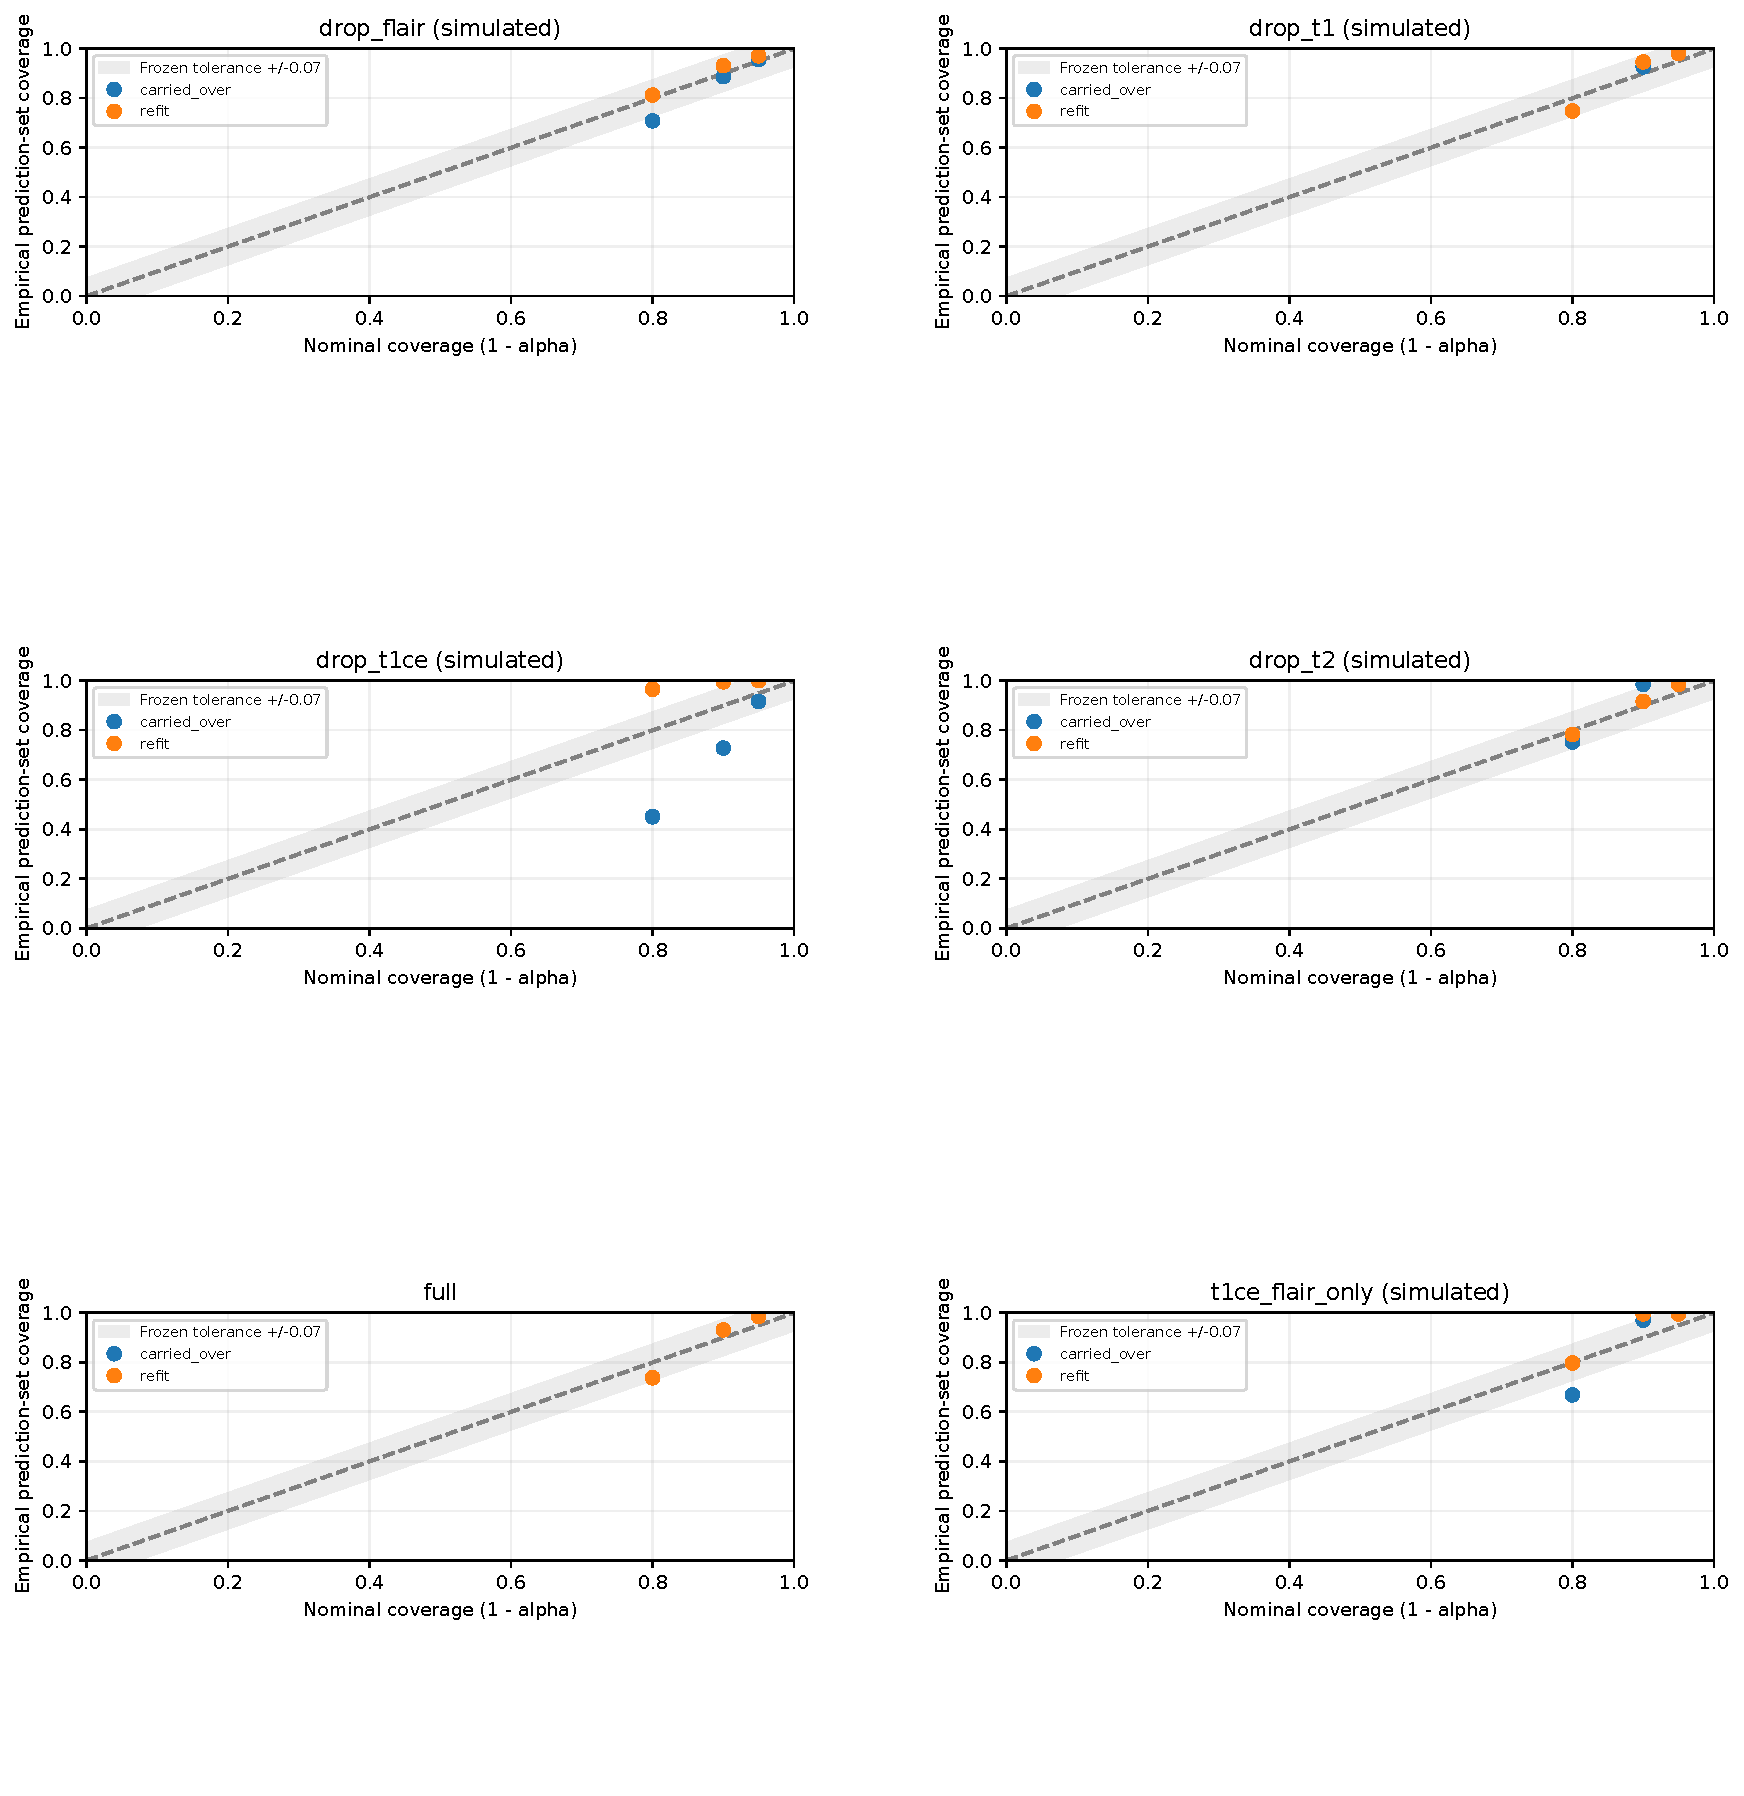
\includegraphics[width=\columnwidth]{figures/fig_3_ucsf_pdgm.pdf}
\caption{Nominal against empirical conformal set coverage on UCSF-PDGM by condition, carried-over quantiles.}
\label{fig:cov}
\end{figure}

\subsection{Calibration across cohorts (RQ3)}
Temperature-scaled ECE was \numIntEceMTwo{} (bootstrap \numIntEceMTwoLo{} to \numIntEceMTwoHi{}) internally and \numExtEceMTwo{} (\numExtEceMTwoLo{} to \numExtEceMTwoHi{}) externally; Brier was \numIntBrierMTwo{} and \numExtBrierMTwo{}. We found no degradation from internal to external data, and the intervals overlap. No family test addresses this contrast, so the statement is descriptive. Temperature scaling did not lower ECE on either cohort (raw ECE \numIntEceMOne{} internally and \numExtEceMOne{} externally). The raw Brier score on UCSF-PDGM was lower than the scaled one by \numExtDTwoAbs, which is statistically detectable and clinically negligible.

\subsection{Ablations}
R7 and R8 did not differ from R2 on UTSW. On UCSF-PDGM R7 had a worse AURC than R2 (difference \numExtETwoDiff, adjusted $p=\numFamXETwoAdj$) and a non-significant AUROC difference (\numExtEOneDiff, adjusted $p=\numFamXEOneAdj$); R8 was not distinguishable from R2 (AUROC difference \numExtEThreeDiff, adjusted $p=\numFamXEThreeAdj$). The evidence for tumour-aware pooling is one AURC contrast on one cohort.

\subsection{Claim summary and multiplicity}
Table~\ref{tab:claims} lists every claim. Of the $\numFamilySize$ family tests, $\numFamilyRejected$ are rejected at $q=0.05$; their adjusted $p$-values sit on the permutation floor times the family size over rank, so they bound the evidence rather than measure it.

\begin{table}[t]
\centering
\caption{Pre-registered claims and their frozen-rule status.}
\label{tab:claims}
\begin{tabular}{lll}
\toprule
Claim & UTSW (internal) & UCSF-PDGM (external) \\
\midrule
C1 & \numStatusCOneInt & --- \\
C2 & \numStatusCTwoInt & --- \\
C3 & --- & \numStatusCThreeExt{} (full); worst \numStatusCThreeWorst \\
C4 & \numStatusCFourInt & \numStatusCFourExt \\
C5 & \numStatusCFiveInt & \numStatusCFiveExt \\
C6 & \numStatusCSixInt & \numStatusCSixExt \\
\bottomrule
\end{tabular}
\end{table}

\section{Discussion}

For this task and these cohorts, abstaining on the least confident cases works on complete input and fails in one specific place. Confidence from the trained network ranks its own errors well enough that dropping the bottom half of cases cuts the error rate to a small fraction of the always-predict rate, on both cohorts. The ranking breaks when T1ce is missing. That sequence carries the enhancement signal that the network relies on, and without it the model is both less accurate and no better at knowing when it is wrong. A deployed system should treat a missing T1ce as a reason to withhold the prediction, not to lower a threshold.

The coverage result is a result about measurement precision. With $\numNInt$ internal and $\numNExt$ external patients, and calibration quantiles from 124 patients, a $0.07$ tolerance cannot be verified at $\alpha=0.1$ or $0.2$. The external point estimates are above nominal at $\alpha=0.05$ and $0.1$ and below it at $\alpha=0.2$, with many empty sets, so there is no simple degrade-only pattern. A larger calibration set is the direct remedy; no feasible split of this cohort reaches the band.

Three results were negative: C2, C4 and (internally) C6 were refuted, and temperature scaling did not improve ECE. We did not re-run, re-tune or re-scope any of them. That the calibration did not degrade externally contradicts the degradation reported for other glioma IDH models; with two cohorts and one architecture we do not claim it generalises.

\subsection{Limitations}
\label{sec:limits}
\begin{itemize}
\item \textbf{Simulated missingness.} All three cohorts are curated four-sequence studies, so missing sequences were simulated by zeroing a channel. That reproduces the information loss but not the real selection mechanism (motion, intolerance, truncated protocols, scanner failure), which may correlate with image quality or disease severity. Every missing-sequence table and caption says ``simulated,'' and the claim wording was not softened after the fact.
\item \textbf{Sample size.} The internal-test split has $\numNIntPos$ mutant patients and the external cohort $\numNExtPos$, so intervals are wide. Coverage-deviation intervals cannot meet the $0.07$ band at $\alpha=0.1$ or $0.2$ (Section~\ref{sec:coverage}).
\item \textbf{Single development institution}, and one external cohort after excluding BraTS-overlapping patients, which changes the label mix. EGD is deferred.
\item \textbf{Labels.} UTSW IDH labels mix immunohistochemistry (66\%) and sequencing (34\%), with a differential false-negative risk for non-R132H variants. Label harmonisation was done by one reviewer. UCSF-PDGM's assay was not independently re-confirmed.
\item \textbf{Calibration split reuse.} The calibration split served early stopping as well as temperature scaling and conformal quantiles, which may make calibration slightly optimistic.
\item \textbf{1p/19q} was examined only internally with a frozen-encoder probe, exploratory, no inferential claim.
\item \textbf{Review depth.} The team was one researcher. Independent checks (Gate D reviews, the recomputation of the external numbers) were done by a second software agent from written contracts, not by a second person. Every reported number matched except for differences traced to a tie-handling ambiguity in the oracle AURC definition, Monte Carlo seed layout and an error in the second agent's own summary, none changing a reported value or claim status.
\item \textbf{Protocol deviation.} The first external manifest omitted R7 and R8; a second signed manifest and run corrected it before any external metric was examined, with no change of method.
\end{itemize}

\section{Conclusion}
Abstention helped where the input was complete and stopped helping when T1ce was missing. Conformal coverage could not be characterised within the pre-registered tolerance at these sample sizes, and calibration did not degrade from the internal to the external cohort. Four of six claims were not supported as stated in at least one cohort, and we report them as such. Code, frozen predictions and a regeneration script allow every number and figure to be rebuilt.

\section*{Declarations}
\textbf{Data.} UTSW-Glioma and UCSF-PDGM are public TCIA collections. No patient-level data or labels are redistributed here.
\textbf{Ethics.} Retrospective analysis of de-identified public data.
\textbf{AI assistance.} [Disclosure wording to be decided by the authors.]
\textbf{Funding and conflicts.} [To be completed.]

\begin{thebibliography}{99}
% D-010: every entry below must be checked against its source before submission.

\bibitem{louis2021} D. N. Louis \emph{et al.}, ``The 2021 WHO classification of tumors of the central nervous system: a summary,'' \emph{Neuro-Oncology}, vol. 23, no. 8, pp. 1231--1251, 2021.

\bibitem{farahani2025} FoundBioNet: S. Farahani \emph{et al.}, MICCAI 2025, doi:10.1007/978-3-032-04981-0\_25.

\bibitem{geifman2017} Y. Geifman and R. El-Yaniv, ``Selective classification for deep neural networks,'' in \emph{Advances in Neural Information Processing Systems}, 2017.

\bibitem{zadorozhny2023} K. Zadorozhny \emph{et al.}, ``Rescuing referral failures during automated diagnosis of domain-shifted medical images,'' arXiv:2311.16766, 2023.

\bibitem{vovk2005} V. Vovk, A. Gammerman, and G. Shafer, \emph{Algorithmic Learning in a Random World}. Springer, 2005.

\bibitem{angelopoulos2023} A. N. Angelopoulos and S. Bates, ``Conformal prediction: a gentle introduction,'' \emph{Foundations and Trends in Machine Learning}, vol. 16, no. 4, 2023.

\bibitem{angelopoulos2024crc} A. N. Angelopoulos, S. Bates, A. Fisch, L. Lei, and T. Schuster, ``Conformal risk control,'' in \emph{International Conference on Learning Representations}, 2024.

\bibitem{liang2026risen} RISEN: Liang \emph{et al.}, \emph{European Radiology}, 2026, doi:10.1007/s00330-026-12622-4.

\bibitem{liu2026gmmas} GMMAS: Liu \emph{et al.}, \emph{Medicine Advances}, 2026, doi:10.1002/med4.70064.

\bibitem{yogananda2025} C. G. B. Yogananda \emph{et al.}, ``Bridging the clinical gap: confidence informed IDH prediction in brain gliomas using MRI and deep learning,'' \emph{Neuro-Oncology Advances}, vol. 7, no. 1, vdaf142, 2025.

\bibitem{elyassirad2026} D. Elyassirad \emph{et al.}, ``Uncertainty-aware IDH mutation status classification with conformal prediction,'' \emph{J. Imaging Informatics in Medicine}, vol. 39, pp. 1217--1224, 2026.

\bibitem{liang2024selective} Liang, Peng, and Sun, ``Selective classification under distribution shifts,'' \emph{Transactions on Machine Learning Research}, 2024.

\bibitem{guo2017} C. Guo, G. Pleiss, Y. Sun, and K. Q. Weinberger, ``On calibration of modern neural networks,'' in \emph{Proc. ICML}, 2017.

\bibitem{gal2016} Y. Gal and Z. Ghahramani, ``Dropout as a Bayesian approximation: representing model uncertainty in deep learning,'' in \emph{Proc. ICML}, 2016.

\bibitem{lakshminarayanan2017} B. Lakshminarayanan, A. Pritzel, and C. Blundell, ``Simple and scalable predictive uncertainty estimation using deep ensembles,'' in \emph{Advances in Neural Information Processing Systems}, 2017.

\bibitem{reddy2026utsw} Reddy \emph{et al.}, UTSW-Glioma, \emph{Scientific Data}, 2026, doi:10.1038/s41597-026-07274-4.

\bibitem{calabrese2022ucsf} E. Calabrese \emph{et al.}, ``The University of California San Francisco preoperative diffuse glioma MRI dataset,'' \emph{Radiology: Artificial Intelligence}, 2022, doi:10.1148/ryai.220058.

\bibitem{isensee2019hdbet} F. Isensee \emph{et al.}, ``Automated brain extraction of multisequence MRI using artificial neural networks,'' \emph{Human Brain Mapping}, vol. 40, no. 17, pp. 4952--4964, 2019.

\bibitem{tustison2010n4} N. J. Tustison \emph{et al.}, ``N4ITK: improved N3 bias correction,'' \emph{IEEE Trans. Med. Imaging}, vol. 29, no. 6, pp. 1310--1320, 2010.

\bibitem{myronenko2019segresnet} A. Myronenko, ``3D MRI brain tumor segmentation using autoencoder regularization,'' in \emph{BrainLes 2018}, Springer, 2019.

\bibitem{cardoso2022monai} M. J. Cardoso \emph{et al.}, ``MONAI: an open-source framework for deep learning in healthcare,'' arXiv:2211.02701, 2022.

\bibitem{loshchilov2019adamw} I. Loshchilov and F. Hutter, ``Decoupled weight decay regularization,'' in \emph{Proc. ICLR}, 2019.

\bibitem{hanley1982} J. A. Hanley and B. J. McNeil, ``The meaning and use of the area under a receiver operating characteristic (ROC) curve,'' \emph{Radiology}, vol. 143, no. 1, pp. 29--36, 1982.

\bibitem{delong1988} E. R. DeLong, D. M. DeLong, and D. L. Clarke-Pearson, ``Comparing the areas under two or more correlated receiver operating characteristic curves: a nonparametric approach,'' \emph{Biometrics}, vol. 44, no. 3, pp. 837--845, 1988.

\bibitem{benjamini1995} Y. Benjamini and Y. Hochberg, ``Controlling the false discovery rate: a practical and powerful approach to multiple testing,'' \emph{J. R. Stat. Soc. B}, vol. 57, no. 1, pp. 289--300, 1995.

\bibitem{borges2024} B. L. C. Borges, B. M. Pacheco, and D. Silva, ``Selective prediction for semantic segmentation using post-hoc confidence estimation and its performance under distribution shift,'' arXiv:2402.10665, 2024.

\bibitem{hirsch2024} R. Hirsch and J. Goldberger, ``A conformalized learning of a prediction set with applications to medical imaging classification,'' arXiv:2408.05037, 2024.

\bibitem{lu2023} C. Lu, Y. Yu, S. P. Karimireddy, M. I. Jordan, and R. Raskar, ``Federated conformal predictors for distributed uncertainty quantification,'' in \emph{Proc. ICML}, PMLR 202, pp. 22942--22964, 2023.

\bibitem{cheung2024} M. Y. Cheung, T. J. Netherton, L. E. Court, A. Veeraraghavan, and G. Balakrishnan, ``Metric-guided image reconstruction bounds via conformal prediction,'' arXiv:2404.15274, 2024.

\bibitem{dorfner2025} F. J. Dorfner, J. B. Patel, J. Kalpathy-Cramer, E. R. Gerstner, and C. P. Bridge, ``A review of deep learning for brain tumor analysis in MRI,'' \emph{npj Precision Oncology}, vol. 9, art. 2, 2025.

\bibitem{ren2025} R. Ren \emph{et al.}, ``Federated radiomics analysis of preoperative MRI across institutions: toward integrated glioma segmentation and molecular subtyping,'' \emph{Frontiers in Radiology}, vol. 5, 1648145, 2025.

\bibitem{liu2026dare} Y. Liu \emph{et al.}, ``DARE-FUSE: domain aligned evidence guided learning for joint brain tumor MRI segmentation and classification,'' \emph{npj Digital Medicine}, vol. 9, art. 178, 2026.

\bibitem{yagis2021} E. Ya\u{g}{\i}\c{s} \emph{et al.}, ``Effect of data leakage in brain MRI classification using 2D convolutional neural networks,'' \emph{Scientific Reports}, vol. 11, art. 22544, 2021.

\end{thebibliography}

\end{document}
